\documentclass[border=5pt]{standalone}
\usepackage{tikz}
\usepackage{amsmath}
\usetikzlibrary{positioning, arrows.meta, calc, fit, backgrounds}

% --- Color Scheme (Blue-Gray) ---
\definecolor{bgPrimary}{HTML}{DAE8FC}
\definecolor{bgSecondary}{HTML}{E8EEF7}
\definecolor{bgAccent}{HTML}{B3CDE3}
\definecolor{bgInput}{HTML}{F0F4F8}
\definecolor{borderPrimary}{HTML}{6C8EBF}
\definecolor{borderAccent}{HTML}{3A6EA5}
\definecolor{arrowColor}{HTML}{4A6A8A}
\definecolor{textMain}{HTML}{2C3E50}
\definecolor{textLight}{HTML}{7F8C8D}
\definecolor{bgHighlight}{HTML}{FFF3CD}

% --- Styles ---
\tikzset{
  module/.style={
    draw=borderPrimary, fill=bgPrimary, rounded corners=4pt,
    minimum width=2.5cm, minimum height=1.0cm,
    font=\sffamily\small, text=textMain, line width=0.6pt, align=center,
  },
  novelmodule/.style={
    draw=borderAccent, fill=bgAccent, rounded corners=4pt,
    minimum width=2.5cm, minimum height=1.0cm,
    font=\sffamily\small\bfseries, text=textMain, line width=1.0pt, align=center,
  },
  iobox/.style={
    draw=borderPrimary, fill=bgInput, rounded corners=3pt,
    minimum width=2cm, minimum height=0.8cm,
    font=\sffamily\small, text=textMain, line width=0.5pt, align=center,
  },
  plusnode/.style={
    circle, draw=borderPrimary, fill=bgSecondary,
    inner sep=0pt, minimum size=16pt,
    font=\sffamily\scriptsize\bfseries, text=textMain, line width=0.5pt,
  },
  stdarrow/.style={
    -{Stealth[length=5pt, width=4pt]}, line width=0.6pt, color=arrowColor,
  },
}

\begin{document}
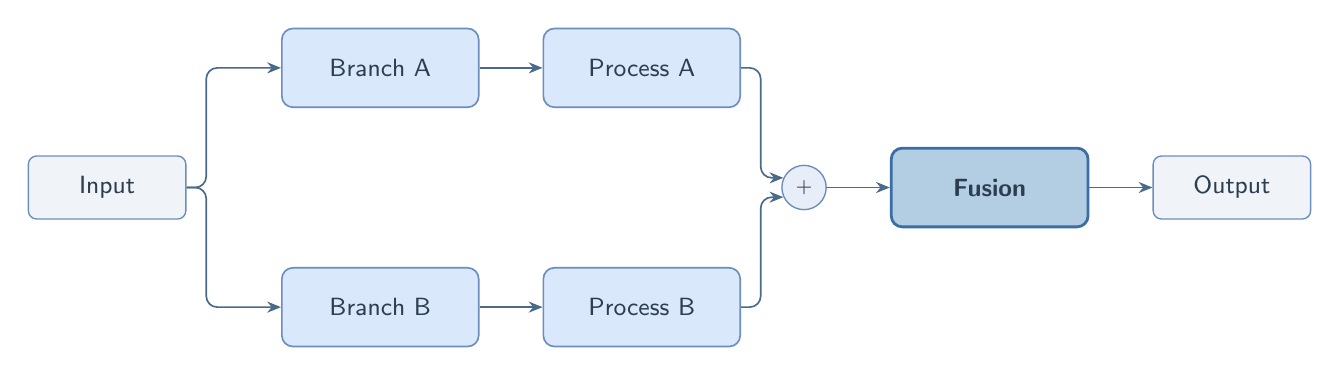
\begin{tikzpicture}

  % --- Input ---
  \node[iobox] (input) {Input};

  % --- Branch A (top) ---
  \node[module, above right=0.6cm and 1.2cm of input] (brA) {Branch A};
  \node[module, right=0.8cm of brA] (procA) {Process A};

  % --- Branch B (bottom) ---
  \node[module, below right=0.6cm and 1.2cm of input] (brB) {Branch B};
  \node[module, right=0.8cm of brB] (procB) {Process B};

  % --- Merge ---
  % Place merge node at x = procA.east + 0.8cm, y = midpoint of procA and procB
  \coordinate (midY) at ($(procA.center)!0.5!(procB.center)$);
  \coordinate (mergeX) at ($(procA.east)+(0.8cm, 0)$);
  \node[plusnode] (merge) at (mergeX |- midY) {$+$};

  % --- Post-merge ---
  \node[novelmodule, right=0.8cm of merge] (fuse) {\textbf{Fusion}};
  \node[iobox, right=0.8cm of fuse] (output) {Output};

  % --- Arrows ---
  \draw[stdarrow, rounded corners=4pt] (input.east) -- ++(0.25cm, 0) |- (brA.west);
  \draw[stdarrow, rounded corners=4pt] (input.east) -- ++(0.25cm, 0) |- (brB.west);
  \draw[stdarrow] (brA)  -- (procA);
  \draw[stdarrow] (brB)  -- (procB);
  \draw[stdarrow, rounded corners=4pt] (procA.east) -- ++(0.25cm, 0) |- (merge.155);
  \draw[stdarrow, rounded corners=4pt] (procB.east) -- ++(0.25cm, 0) |- (merge.205);
  \draw[stdarrow] (merge) -- (fuse);
  \draw[stdarrow] (fuse) -- (output);

\end{tikzpicture}
\end{document}
